\documentclass[border=0pt]{standalone}
\usepackage{amsmath}
\usepackage[usenames,dvipsnames]{xcolor}
\usepackage{graphicx}

%%font
\usepackage{euler}
\usepackage[OT1]{eulervm}
\renewcommand{\rmdefault}{pplx}

\usepackage{tikz}
\tikzset{roundnode/.style={circle,draw=black,fill=blue!20}}
\definecolor{TortugaColor}{rgb}{0.1,0.4,0.3}
\definecolor{Totemblue}{HTML}{09182F}
\definecolor{Totemred}{HTML}{2B030B}
\definecolor{Totemyellow}{HTML}{AD901B}
\usetikzlibrary{intersections}
%\usetikzlibrary{fadings}
\usetikzlibrary{arrows}
%\usetikzlibrary{arrows.meta}
%\usetikzlibrary{decorations}
\usetikzlibrary{decorations.pathmorphing}
\usetikzlibrary{decorations.text}
%\usetikzlibrary{fit}
%\usetikzlibrary{calc}
%\usetikzlibrary{through}
%\usetikzlibrary{positioning}
%\usetikzlibrary{graphs}
%\usetikzlibrary{mindmap}
%\usetikzlibrary{backgrounds}
\usetikzlibrary{calligraphy}
\usepgfmodule{nonlineartransformations}
\usetikzlibrary{curvilinear}
\makeatletter
\def\polartransformation{%
% \pgf@x will contain the radius
% \pgf@y will contain the distance
\pgfmathsincos@{\pgf@sys@tonumber\pgf@x}%
% pgfmathresultx is now the cosine of radius and
% pgfmathresulty is the sine of radius
\pgf@x=\pgfmathresultx\pgf@y%
\pgf@y=\pgfmathresulty\pgf@y%
}
\makeatother

\pgfdeclarelayer{background}
\pgfdeclarelayer{alpha}
\pgfdeclarelayer{beta}
\pgfsetlayers{background,alpha,main,beta}

%%pic Totu
\tikzset{
totu/.pic={
\begin{scope}[scale=0.2]
\pgfmathsetmacro{\legwidth}{0.4*0.2}
\draw[fill=green!60!black!30] (0,0.8) circle [x radius=0.3,y radius=0.4];
\foreach \i in {-1,1}{
\begin{scope}[xscale=\i]
\path (0.8,0) edge[draw=green!60!black!30,line width=\legwidth cm,line cap=round,bend left] ++(0.6,0);
\path (0.6,-1) edge[draw=green!60!black!30,line width=\legwidth cm,line cap=round] ++ (0.4,-0.4);
\end{scope}
}
\draw (0,-1.4) edge[draw=green!60!black!30,line width=\legwidth cm,line cap=round] ++ (0,-0.4);
\draw[fill=green!60!black,rounded corners] (1,0) -- (0,0.5) -- (-1,0) -- (-0.8,-1.2) -- (0,-1.6) -- (0.8,-1.2) -- cycle;
\end{scope}
}}

%%pic Rescuer
\tikzset{
Rescuer/.pic={
\begin{scope}[shift={(0.5,-2)}]
\draw[fill=black!20!red!60!yellow] (-7,-0.8) -- (-6.7,-1.2) -- (-6,-1.2) -- (-5.7,-0.8) .. controls +(-0.3,-0.1) and +(0.3,-0.1) ..  cycle;
\end{scope}
}}

%%pic SatanHeart
\tikzset{
SatanHeart/.pic={
\pgfmathsetmacro{\SatanHradius}{1}
\pgfmathsetmacro{\LSatanHradius}{1.05}
\begin{scope}[very thick]
\draw[gray!80!blue, line width=2pt] (0,0) circle[radius=\LSatanHradius cm];
\draw[gray!80!blue] (-90:\SatanHradius) -- (-306:\SatanHradius) -- (-162:\SatanHradius) -- (-378:\SatanHradius) -- (-234:\SatanHradius) -- cycle;
\end{scope}
}}

%%pic Stone Gate
\tikzset{
stonegate/.pic={
\begin{scope}[gray]
\draw[fill,draw=none,rounded corners] (-1.3,-0.3) rectangle (-0.7,2);
\draw[fill,draw=none,rounded corners] (0.7,-0.3) rectangle (1.3,2);
\draw[fill,draw=none] (0,2) ellipse[x radius=2cm, y radius=0.3cm];
\end{scope}
}}

%%pic Ateles Zombia
\tikzset{
zombia/.pic={
\pgfmathsetmacro{\zombiascale}{0.2}
\begin{scope}[scale=\zombiascale]
\pgfmathsetmacro{\zombiawidth}{\zombiascale *0.3 cm}
\pgfmathsetmacro{\zombiabigcorner}{\zombiascale *4 pt}
\pgfmathsetmacro{\zombiasmallcorner}{\zombiascale *0.2 cm}
\begin{scope}[gray!40, rounded corners=\zombiabigcorner, line width=\zombiawidth, line cap=round]
%\node[circle,draw,thin] at (0,0) {};
\draw [fill,thin] (-1.9,0.4) circle [radius=0.3cm];
\draw (-1.8,0.1) -- (-2.2,-0.3) -- (-2.7,-0.6);
\draw (-1.8,0.1) -- (-1.6,-0.8) -- ++ (0.1,-0.1);
\draw (-1.8,0.1) -- (-0.9,0.1) -- (0.4,0.8);
\draw[rounded corners=\zombiasmallcorner] (0.4,0.8) -- ++ (0.3,0.2) -- ++ (0.2,-0.2);
\draw (0.7,1) -- (0.9,1.3) -- (1,2.5) -- (1.3,3) -- (1.8,2.9);
\draw (0.9,0.8) -- (0.9,0.5) -- (0.95,-0.3) -- (0.8,-1.1);
\draw (0.8,0.8) -- (0.4,0.6) -- (0,-0.7) -- ++(-0.2,-0.2);
\end{scope}
\end{scope}
}
}

\parindent=0pt

\begin{document}
%%2017NewYear
%% 16:9
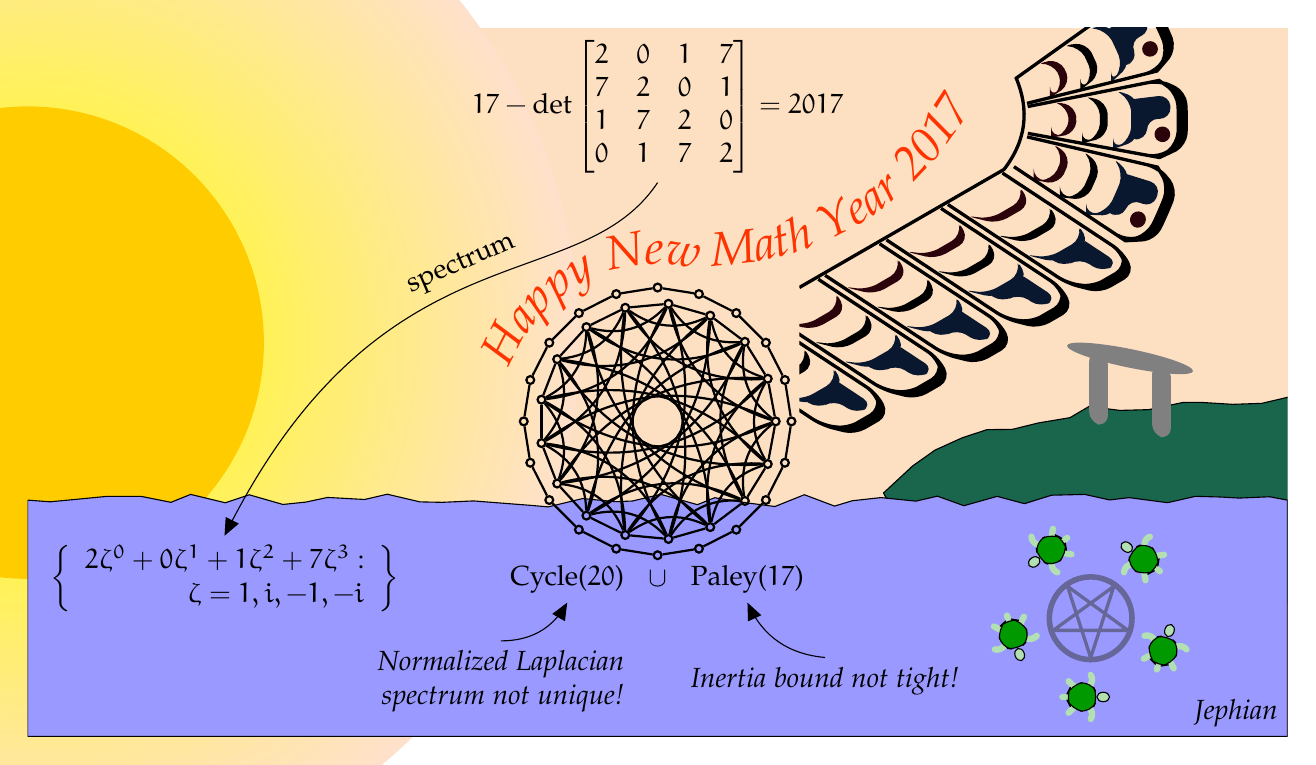
\begin{tikzpicture}
\coordinate (Jamaica) at (-8,-4);
\coordinate (Dominican) at (8,-4);
\coordinate (Cuba) at (-8,5);
\coordinate (TurksCaicos) at (8,5);
\coordinate (Tortuga) at (0,0);
\clip (Jamaica) rectangle (TurksCaicos);

%%Help Lines
\begin{pgfonlayer}{beta}
%\draw [step=1, black!50, thin] (Jamaica) grid (TurksCaicos);
%\draw (0,0) circle [radius=0.5cm];
\end{pgfonlayer}

%%background Layer
\begin{pgfonlayer}{background}
\fill [yellow!40!red!20!white] (-8,-4) rectangle (8,5);
\coordinate (suncenter) at (0,1 -| Jamaica);
\pgfmathsetmacro{\sunradius}{3};
\pgfmathsetmacro{\nolight}{7};
\shade [inner color=yellow, outer color=yellow!40!red!20!white] (suncenter) circle [radius=\nolight cm];
\path [fill=red!20!yellow] (suncenter) circle [radius=\sunradius cm];
\end{pgfonlayer}


%%Main Layer
\begin{pgfonlayer}{main}
%%Tortuga
\draw[fill=TortugaColor] decorate[decoration={name=random steps}] {(0,-1-|Dominican) ellipse [x radius=5cm, y radius=1.3cm]};
%%Sea
\draw[fill=blue!40,name path=sealevel] decorate[decoration={name=random steps}] {(0,-1 -| Jamaica) -- (0,-1 -| Dominican)} -- (Dominican) -- (Jamaica) -- cycle;
%%StoneGate
\pic[scale=0.4,yslant=-0.2] at (6,0) {stonegate};
%%SatanHeart
\pic[scale=0.5] at (5.5,-2.5) {SatanHeart};
%%totus swimming
\begin{scope}[xshift=5.5cm, yshift=-2.5cm]
\foreach \ang in {54,126,198,270,342}{
\pic[rotate=\ang] at (\ang:1) {totu};
}
\end{scope}
%%C20 union Paley 17
\begin{scope}[thick, every node/.style={draw,circle,inner sep=1pt}]
%%C20
  \foreach \i in {0,...,19}{
    \pgfmathsetmacro{\ang}{\i*18}
    \node (c\i) at (\ang:1.7) {};
  }
  \foreach \i in {0,...,19}{
    \pgfmathsetmacro{\iplusone}{int(mod(\i+1,20))}
    \draw (c\i)--(c\iplusone);
  }
%%Paley17
  \foreach \i in {0,...,16}{
    \pgfmathsetmacro{\ang}{\i*360/17}
    \node (p\i) at (\ang:1.5) {};
  }
  \foreach \gen in {1,2,4,8}{
    \pgfmathsetmacro{\type}{\gen==1? "":"bend left"}
    \foreach \i in {0,...,16}{
      \pgfmathsetmacro{\inext}{int(mod(\i+\gen,17))}
      \path[\type] (p\i) edge (p\inext);
    }
  }
\end{scope}
%%Captions
\node at (0,-2) {$\cup$};
\node[left] (C20) at (-0.3,-2) {Cycle($20$)};
\node[right] (P17) at (0.3,-2) {Paley($17$)};
\node[left,align=right] (normalizedL) at (-0.3,-3.3) {\it Normalized Laplacian\\\it spectrum not unique!};
\node[right] (inertiabound) at (0.3,-3.3) {\it Inertia bound not tight!};
\draw[-triangle 45] (normalizedL.north) to[bend right] (C20.south);
\draw[-triangle 45] (inertiabound.north) to[bend left] (P17.south);

\begin{scope}
\clip (1.8,-0.5) rectangle (TurksCaicos);
\draw[very thick] (1.8,1.7) -- (4.4,3.2) to[bend right] (4.55,4.37); 
%%ThuderBirdWing
\begin{scope}[xshift=0.5cm,yshift=1cm, rotate=30,xslant=-0.5]
%%StraightFeather
\foreach \i in {0,...,4}{
\pgfmathsetmacro{\newx}{\i*0.9}
\begin{scope}[xshift=\newx cm,xscale=0.8]
  \draw[draw=none,rounded corners, fill=Totemred] (0,-0.3) -- (0.2,-0.6) -- (0.8,-0.6) -- (1,-0.3) -- (0.8,-0.5) -- (0.2,-0.5) -- cycle;
  \draw[draw=none,rounded corners, fill=black] (0,-0.7) -- (0.2,-1) -- (0.8,-1) -- (1,-0.7) -- (0.8,-0.9) -- (0.2,-0.9) -- cycle;
  \draw[draw=none,rounded corners, fill=Totemblue] (0,-1.1) -- (0.2,-1.4) -- (0.8,-1.4) -- (1,-1.1) -- (0.8,-1.3) -- (0.2,-1.3) -- cycle;
  \draw[draw=none, rounded corners, fill=Totemblue] (0.2,-1.35) -- (0.2,-1.5) -- (0.5,-1.5) -- (0.5,-1.8) -- (0.8,-1.8) -- (0.8,-1.35);  
  \draw[rounded corners,very thick, fill=black] (0,0) -- (0,-1.7) -- (0.2,-2) -- (0.8,-2) -- (1,-1.7) -- (1,0) -- (1,-1.7) -- (0.8,-1.9) -- (0.2,-1.9) -- (0,-1.7) -- cycle;
\end{scope}
}
\end{scope} %%Straightpart
%%%Morphed feather
{\pgfsetcurvilinearbeziercurve
  {\pgfpointadd{\pgfpointpolar{-34}{2cm}}{\pgfpoint{37mm}{38mm}}}
  {\pgfpointadd{\pgfpointpolar{-4}{2.3cm}}{\pgfpoint{37mm}{38mm}}}
  {\pgfpointadd{\pgfpointpolar{26}{2.3cm}}{\pgfpoint{37mm}{38mm}}}
  {\pgfpointadd{\pgfpointpolar{56}{2cm}}{\pgfpoint{37mm}{38mm}}}
  \makeatletter
\pgftransformnonlinear{\pgfpointcurvilinearbezierorthogonal\pgf@x\pgf@y}%
\makeatother
%\draw (0,-1) grid (3,1);
\foreach \i in {0,1,2}{
\pgfmathsetmacro{\newx}{0.9*\i}
\begin{scope}[xshift=\newx cm,yshift=1cm,xscale=0.8] %%Beforemorph
\draw[draw=none,rounded corners, fill=Totemred] (0,-0.3) -- (0.2,-0.6) -- (0.8,-0.6) -- (1,-0.3) -- (0.8,-0.5) -- (0.2,-0.5) -- cycle;
  \draw[draw=none,rounded corners, fill=black] (0,-0.7) -- (0.2,-1) -- (0.8,-1) -- (1,-0.7) -- (0.8,-0.9) -- (0.2,-0.9) -- cycle;
  \draw[draw=none,rounded corners, fill=Totemblue] (0,-1.1) -- (0.2,-1.4) -- (0.8,-1.4) -- (1,-1.1) -- (0.8,-1.3) -- (0.2,-1.3) -- cycle;
  \draw[draw=none, rounded corners, fill=Totemblue] (0.2,-1.35) -- (0.2,-1.5) -- (0.5,-1.5) -- (0.5,-1.8) -- (0.8,-1.8) -- (0.8,-1.35);  
  \draw[rounded corners,very thick, fill=black] (0,0) -- (0,-1.7) -- (0.2,-2) -- (0.8,-2) -- (1,-1.7) -- (1,0) -- (1,-1.7) -- (0.8,-1.9) -- (0.2,-1.9) -- (0,-1.7) -- cycle;
  \draw[draw=none,fill=Totemred] (0.3,-1.7) circle[radius=1mm];
\end{scope} %%Beforemorph
}}
\end{scope} %%Clip
\end{pgfonlayer}


%%beta layer
\begin{pgfonlayer}{beta}

%%17determinant
  \node (17det) at (0,4) {$17-\det\begin{bmatrix}
    2 & 0 & 1 & 7 \\
    7 & 2 & 0 & 1 \\
    1 & 7 & 2 & 0 \\
    0 & 1 & 7 & 2 \\
    \end{bmatrix}=2017
    $};
%%17FastFourierTransform
  \node (17spec) at (-5.5,-2) {$\left\{\begin{array}{r}
    2\zeta^0+0\zeta^1+1\zeta^2+7\zeta^3:\\
    \zeta=1,i,-1,-i\\
    \end{array}\right\}
  $};
\draw[-triangle 45] (17det.south) .. controls +(-1,-1.5) and +(2,4) .. node[midway,sloped,above] {spectrum} (17spec.north);
%%Happy New Math Year
%\node[red!80!yellow] at (1,2.2) {\Huge \it Happy New Math Year 2017};
\draw[decorate,decoration={text along path,text={|\color{red!80!yellow} \LARGE \it|Happy New Math Year 2017}}] (160:2) arc (160:80:2) to[bend right] (4,4);

%%Signature
\node[yshift=0.3cm,left] at (Dominican) {\it Jephian};

\end{pgfonlayer}




\end{tikzpicture}
\end{document}
%%\draw=\path[draw]
%%\clip=\path[clip]
%%\graph=\path[graph]
%%bend right ~ bend right=30 ~ in,out=right30, left 30
%%(left:2)=(180:2)
%%left ~ anchor=east ~ anchor 0
%For updating 2.10 to 3.0.0
%after moving the folder, it requires 
%sudo texhash 
% to make it work.
%%To convert to jpg: compile the pdf first, and then use the command below
%% convert -density 300 file.pdf -quality 90 file.jpg
